\section{Comparação $\beta^{3}$-\gls{IRT} e $\beta^4$-\gls{IRT}}

% \section{Introdução}
Este capítulo apresenta uma análise empírica comparativa entre os modelos $\beta^{3}$-\gls{IRT} e $\beta^{4}$-\gls{IRT} , com foco na estabilidade do processo de estimação e na capacidade de recuperação dos parâmetros latentes. O objetivo é investigar como o problema de não-identificabilidade do $\beta^{3}$-\gls{IRT} se manifesta na prática e em que medida a reformulação proposta no $\beta^{4}$-\gls{IRT}  contribui para mitigar seus efeitos.

\section{Definição do Experimento}

Para avaliar o impacto da simétria  na recuperação de parâmetros, foram amostrados $1000$ valores de habilidades, dificuldades e discriminações a partir das distribuições a priori definidas no modelo, na equação \ref{eq:model_def}, assumindo variância inicial $\sigma_{0}^2 = 1$.

A partir desses parâmetros latentes, foi gerada uma matriz de respostas de dimensão $1000 \times 1000$. Para cada par respondente e item $(i, j)$, a resposta observada $p_{ij}$ foi obtida como a média de $100$ amostras provenientes da distribuição $Beta$ correspondente.

Em seguida, ajustamos os modelos $\beta^3$-\gls{IRT} e $\beta^3$-\gls{IRT} via Máxima Verossimilhança utilizando gradiente descendente por $50.000$ iterações. Para analisar o impacto da simétria, realizamos diferentes estratégias de inicialização, incluindo períodos iniciais com discriminações fixadas.

A avaliação foi realizada por meio de gráficos de dispersão comparando valores reais e estimados dos parâmetros. Instâncias cujo sinal da discriminação foi invertido após a estimação foram destacadas em vermelho.

Além do experimento ilustrativo com uma única matriz 
$1000\times1000$, foi conduzido um experimento de Monte Carlo com $30$ amostras independentes para avaliar o desempenho dos modelos sob diferentes configurações de dados.

Foram consideradas três configurações de tamanho de conjunto:

\begin{itemize}
    \item $N = 100$ itens e $M = 20$ respondentes;
    \item $N = 100$ itens e $M = 100$ respondentes;
    \item $N = 300$ itens e $M = 50$ respondentes;
\end{itemize}

Para cada replicação e cada configuração do experimento, as habilidades $\theta_i$ e as dificuldades $\delta_j$ foram amostradas de uma distribuição $\Beta(1,1)$, enquanto as discriminações $a_j$ foram geradas a partir de uma distribuição $N(1,1)$. Cada resposta $p_{ij}$ foi construída como a média de $100$ amostras provenientes da distribuição Beta parametrizada pelos valores do modelo. A matriz de respostas $P$ resultante foi utilizada para ajustar os modelos $\beta^3$-\gls{IRT} e $\beta^4$-\gls{IRT}, considerando $50.000$ épocas de treinamento, $1.000$ iterações iniciais com as discriminações fixadas e os demais hiperparâmetros mantidos em seus valores padrão.

Utilizando bootstrap \cite{hesterberg2011bootstrap}, calculamos o intervalo de confiança de 95\% para a correlação de Pearson $\rho$ entre os valores estimados e os valores originais dos parâmetros. O objetivo é avaliar o quão bem os modelos conseguem recuperar a ordenação original dos parâmetros. Isso significa que, para valores positivos e estatisticamente significativos de $\rho$, a relação de ordem entre os parâmetros tende a ser preservada (por exemplo, se $\theta_1 > \theta_2$, então espera-se que $\hat{\theta}_1 > \hat{\theta}_2$).

Além disso, também consideramos o intervalo de confiança de 95\% para o \gls{RSE}, a fim de avaliar a qualidade das estimativas obtidas por cada modelo. O RSE quantifica a proporção da variância não explicada e é definido como \gls{RSE}$ = 1 - R^2$.

\section{Recuperação de Parâmetros} % para o $\beta^3$-\gls{IRT}}

A Figura \ref{fig:b3-0-init-1000x1000(109)} apresenta a comparação entre os valores originais e os valores estimados para as habilidades, dificuldades e discriminações no modelo $\beta^3$-\gls{IRT}. Observa-se que as discriminações estimadas exibem uma relação sigmoidal invertida em relação aos valores reais, indicando uma distorção sistemática no processo de recuperação dos parâmetros. Para valores extremos, os pontos se afastam significativamente da diagonal, evidenciando maior erro de estimação nessas regiões. Além disso, 109 discriminações tiveram seu sinal invertido durante o processo de estimação.

\begin{figure*}[!htb]
\centering
% \includegraphics[width=\linewidth,trim={0cm 0.cm 12.cm 0.cm},clip]{/doc/assets/scatterplot/b3-e50000_i0.png}
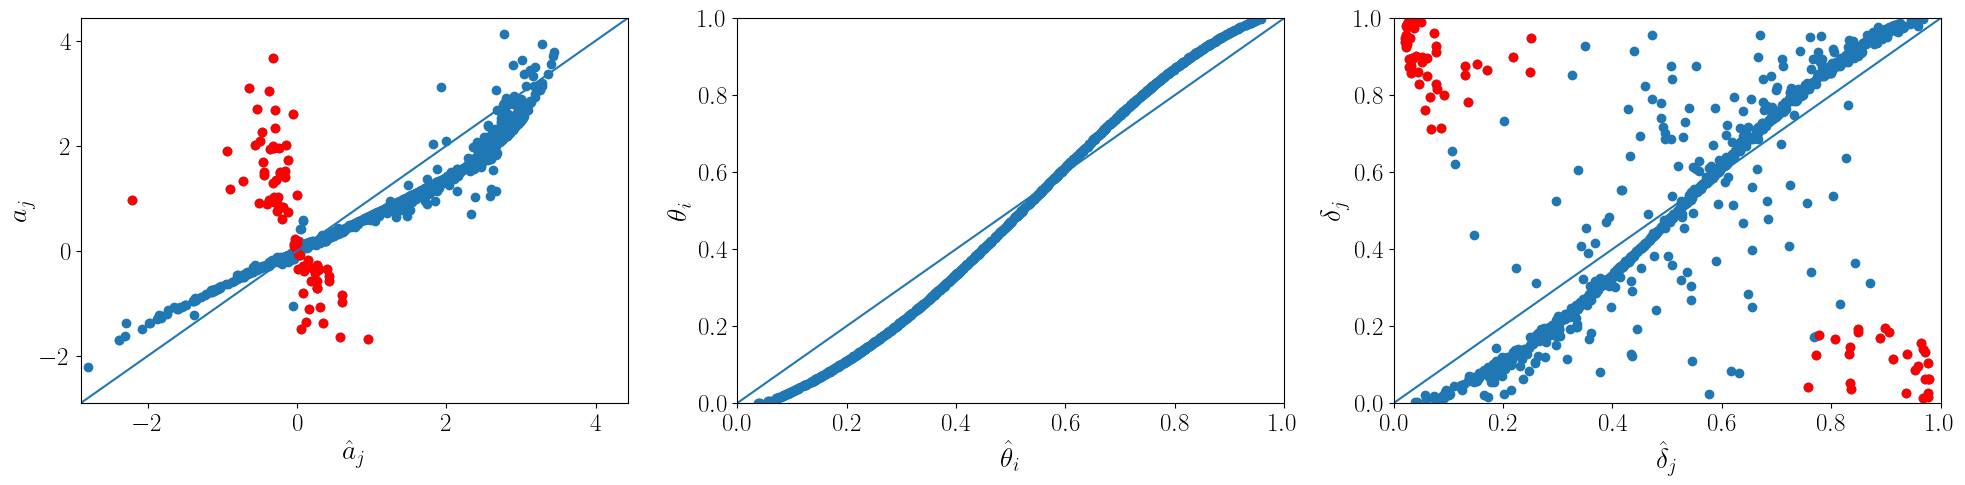
\includegraphics[width=\linewidth,clip]{chapters/fundamentacao/imagens/b3-e50000_i0.png}

\caption{Gráfico de dispersão mostrando as discriminações amostradas (centro), as habilidades (esquerda) e as dificuldades (direita) usadas para gerar uma matriz de resposta de $1.000 \times 1.000$, e suas estimativas produzidas pela $\beta^3$-\gls{IRT}. Os pontos vermelhos nos gráficos de discriminação e dificuldade representam itens cujas discriminações foram estimadas com sinais invertidos ($109$ de $1.000$ discriminações).}
\label{fig:b3-0-init-1000x1000(109)}
\end{figure*}

Essas inversões decorrem diretamente da simétria intrinseca ao modelo, uma vez que uma discriminação com sinal invertido pode ser compensada por ajustes na dificuldade correspondente, mantendo a verossimilhança praticamente inalterada. Como consequência, as dificuldades associadas aos itens com sinal invertido são deslocadas para longe de seus valores verdadeiros. De forma análoga, as habilidades também sofrem deslocamentos, pois o modelo busca compensar os erros estruturais introduzidos nas discriminações. Esse comportamento evidencia que o problema de não-identificabilidade não é apenas uma questão teórica, mas possui impacto direto na qualidade da recuperação dos parâmetros.

% \section{Inicialização para o $\beta^3$-\gls{IRT}}

Uma tentativa de mitigar esse problema consiste em fixar temporariamente as discriminações durante as primeiras iterações do treinamento, permitindo que as habilidades e dificuldades convirjam antes de liberar a otimização do parâmetro $a_j$. Especificamente, ao manter $a_j = 1$ nas $1000$ iterações iniciais, o número de discriminações com sinal invertido foi reduzido de $109$ para $37$, como visto na Figura \ref{fig:b3-1000-init-1000x1000(37)}, indicando uma melhora parcial no comportamento do processo de estimação.

\begin{figure*}[!htb]
\centering
% \includegraphics[width=\linewidth,trim={0cm 0.cm 12.cm 0.cm},clip]{/doc/assets/scatterplot/b3-e50000_i1000.png}
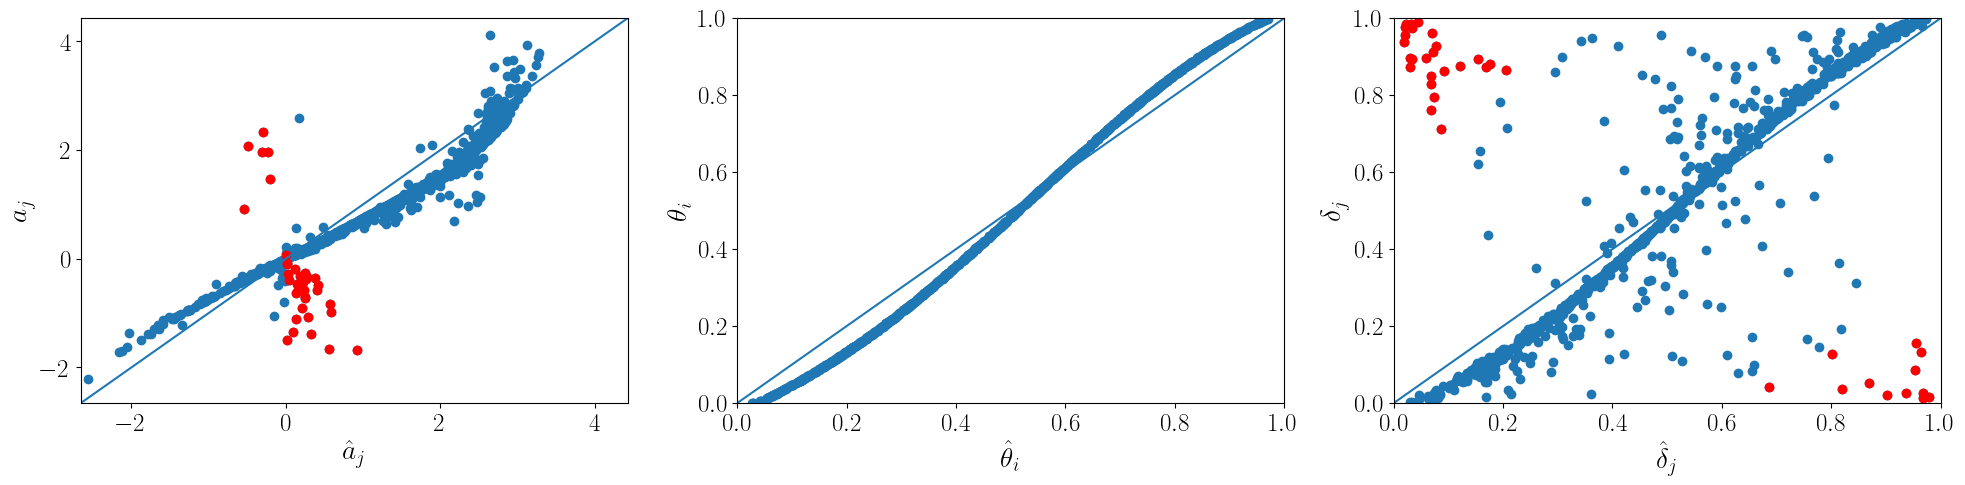
\includegraphics[width=\linewidth,clip]{chapters/fundamentacao/imagens/b3-e50000_i1000.png}
%\\
%
\caption{Gráfico de dispersão mostrando as discriminações amostradas (centro), as habilidades (esquerda) e as dificuldades (direita) usadas para gerar uma matriz de resposta de $1.000 \times 1.000$, e suas estimativas produzidas pela $\beta^3$-\gls{IRT} com $1.000$ inicializações fixas. Os pontos vermelhos nos gráficos de discriminação e dificuldade representam itens cujas discriminações foram estimadas com sinais invertidos ($37$ de $1.000$ discriminações). }
\label{fig:b3-1000-init-1000x1000(37)}
\end{figure*}

Entretanto, essa estratégia não elimina o problema estrutural do modelo. Apesar da redução nas inversões, o modelo permanece vulnerável à sua simétria interna, e inversões de sinal continuam a ocorrer. Esse resultado sugere que a dificuldade não está apenas relacionada à inicialização dos parâmetros, mas sim à própria parametrização do modelo, que permite múltiplas configurações equivalentes em termos de verossimilhança.

% \section{Recuperação de Parâmetros para o $\beta^4$-\gls{IRT} (Sem informação a priori)}

Aplicando o mesmo protocolo experimental ao modelo $\beta^4$-\gls{IRT}, inicialmente considerando apenas a refatoração do parâmetro de discriminação em magnitude e sinal, observa-se uma melhora parcial no processo de recuperação dos parâmetros, conforme ilustrado na Figura \ref{fig:b4-1000-init-1000x1000(77).png}. Com $1.000$ iterações iniciais mantendo o discriminante fixa, 77 discriminações apresentaram inversão de sinal. Embora esse número ainda seja expressivo, ele indica um comportamento distinto em relação ao observado no $\beta^3$-\gls{IRT}.

\begin{figure*}[!htb]
\centering
% \includegraphics[width=\linewidth,trim={0cm 0.cm 12.cm 0.cm},clip]{doc/assets/scatterplot/b4-e50000_i0.png}
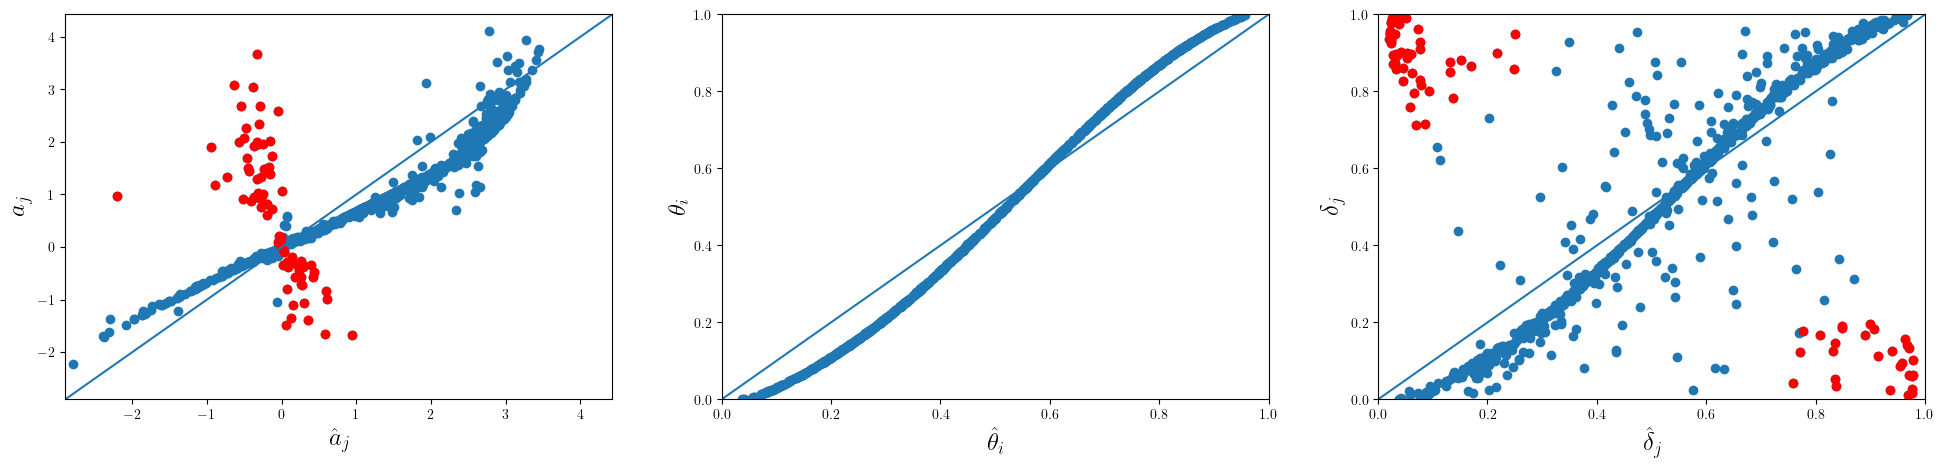
\includegraphics[width=\linewidth,clip]{chapters/fundamentacao/imagens/b4-e50000_i1000_non-prior.png}
%\\
%
\caption{Gráfico de dispersão mostrando as discriminações amostradas (centro), as habilidades (esquerda) e as dificuldades (direita) usadas para gerar uma matriz de resposta de $1.000 \times 1.000$, e suas estimativas produzidas pela $\beta^4$-\gls{IRT} com $1.000$ inicializações fixas. Os pontos vermelhos nos gráficos de discriminação e dificuldade representam itens cujas discriminações foram estimadas com sinais invertidos ($109$ de $1.000$ discriminações). }
\label{fig:b4-1000-init-1000x1000(77).png}
\end{figure*}

Esse resultado evidencia que a simples decomposição $a_j = \omega_j \cdot \tau_j$ não elimina automaticamente a simétria do modelo. Entretanto, diferentemente do $\beta^3$-\gls{IRT}, o $\beta^4$-\gls{IRT} permite impor restrições mais informativas sobre o sinal e a magnitude de forma separada, oferecendo maior controle estrutural sobre o processo de estimação. Essa diferença estrutural é crucial, pois abre caminho para estratégias de identificação mais robustas.

% \section{$\beta^4$-\gls{IRT} com Informação a Priori}

% Explorando a nova parametrização, foram definidos priors sensíveis para cada componente do modelo. As habilidades foram inicializadas a partir da média das respostas de cada indivíduo, enquanto as dificuldades foram definidas com base na média complementar das respostas dos itens. As magnitudes das discriminações foram inicialmente fixadas, e o sinal foi determinado a partir da correlação de Pearson entre as habilidades iniciais e as respostas de cada item, incorporando assim uma informação empírica sobre a direção da relação item-traço latente.

\begin{figure*}[!htb]
\centering
% \includegraphics[width=\linewidth,trim={0cm 0.cm 12.cm 0.cm},clip]{/doc/assets/scatterplot/b3-e50000_i1000.png}
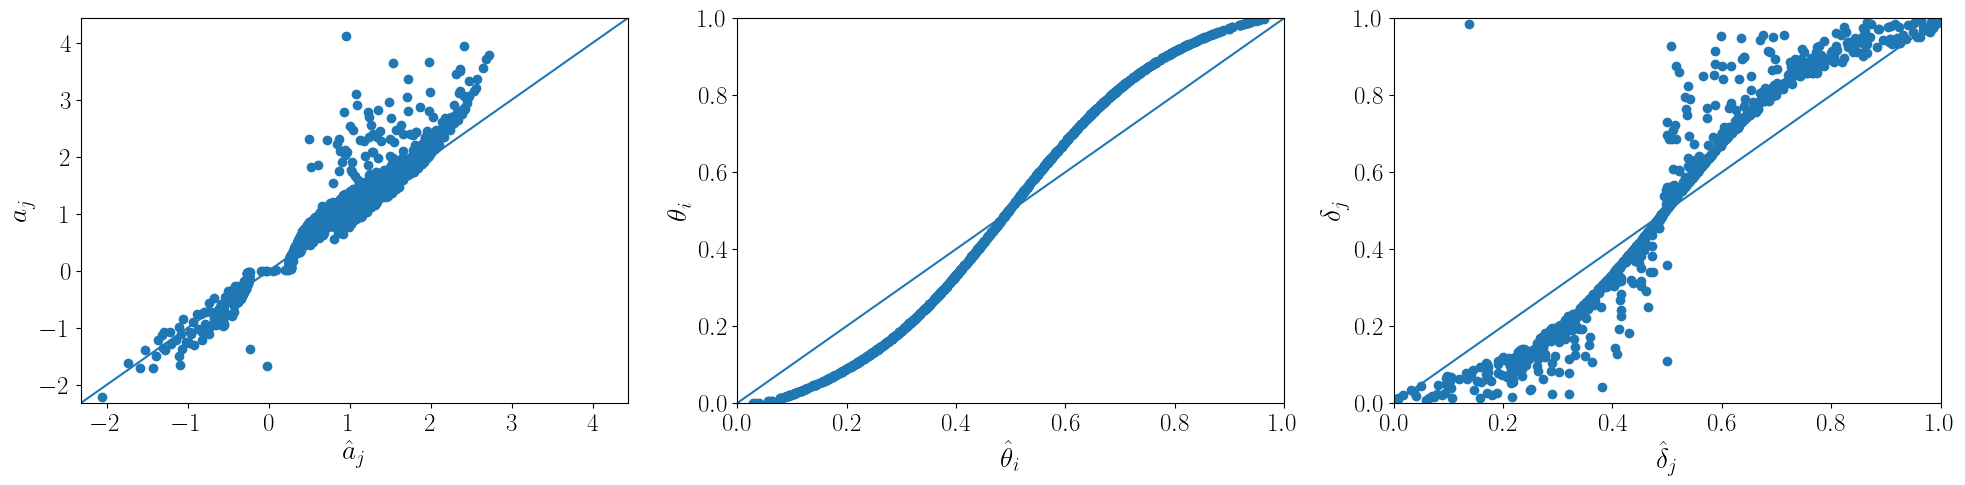
\includegraphics[width=\linewidth,clip]{chapters/fundamentacao/imagens/b4-e50000_i1000.png}
%\\
%
\caption{Gráfico de dispersão mostrando as discriminações amostradas (centro), as habilidades (esquerda) e as dificuldades (direita) usadas para gerar uma matriz de resposta de $1.000 \times 1.000$, e suas estimativas produzidas pela $\beta^3$-\gls{IRT} com $1.000$ inicializações fixas e a melhor informação a priori para cada parâmetro. Os pontos vermelhos nos gráficos de discriminação e dificuldade representam itens cujas discriminações foram estimadas com sinais invertidos ($37$ de $1.000$ discriminações). }

\label{fig:b4-priors-1000-init-1000x1000(0).png}
\end{figure*}

Explorando a nova parametrização, foram definidos priors sensíveis para cada componente do modelo. As habilidades foram inicializadas a partir da média das respostas de cada indivíduo, enquanto as dificuldades foram definidas com base na média complementar das respostas dos itens. As magnitudes das discriminações foram inicialmente fixadas, e o sinal foi determinado a partir da correlação de Pearson entre as habilidades iniciais e as respostas de cada item, incorporando assim uma informação empírica sobre a direção da relação item-traço latente.

Conforme ilustrado na Figura \ref{fig:b4-priors-1000-init-1000x1000(0).png}, com essa estratégia nenhuma discriminação apresentou inversão de sinal ao longo do processo de estimação. Observou-se ainda uma redução significativa da dispersão em torno da diagonal nas comparações entre valores verdadeiros e estimados, além de uma recuperação mais estável das habilidades e dificuldades. O fenômeno de espalhamento anteriormente observado no $\beta^3$-\gls{IRT} deixou de ocorrer. Esse resultado evidencia que a separação explícita entre sinal e magnitude possibilita a introdução de informação estrutural adicional, capaz de quebrar a simétria interna do modelo e melhorar substancialmente sua identificabilidade.

\section{Experimento Monte Carlo}


Para avaliar de forma sistemática a capacidade de recuperação dos parâmetros pelos modelos $\beta^{3}$-\gls{IRT}e $\beta^{4}$-\gls{IRT}, foi conduzido um experimento de Monte Carlo considerando múltiplas replicações e diferentes configurações de tamanho de conjunto de dados. A qualidade das estimativas foi analisada sob três perspectivas complementares. Primeiramente, utilizou-se a correlação de Pearson ($\rho$) entre os valores verdadeiros e estimados dos parâmetros, com intervalos de confiança de 95\% obtidos via bootstrap. Essa métrica permite avaliar a preservação do ordenamento dos parâmetros latentes, aspecto fundamental quando o interesse está na comparação relativa entre habilidades, dificuldades ou discriminações. Em segundo lugar, definimos \gls{RSE} como \gls{RSE}$ = 1 - R^2$, que representa a proporção de variância não explicada pelas estimativas, fornecendo uma medida direta de erro de recuperação. Por fim, avaliou-se a proporção de discriminações estimadas com sinal invertido, também acompanhada de intervalos de confiança de 95\%, uma vez que a inversão de sinais constitui o principal sintoma prático do problema de simétria discutido anteriormente.


% %usar um gerador é uma opção https://www.tablesgenerator.com/
% % observação, segundo a biblioteca tableas não podem ter nenhuma linha vertical


{\color{blue}
\begin{table}[!htb]
    %\centering
\begin{tabular}{ccccc}
\toprule
Amostra & Parâmetro & Modelo & RSE, 95\% CI & $\rho$, 95\% CI \\
\cline{1-5}
\multirow[c]{6}{*}{$N = 100$, $M = 100$} & \multirow[c]{2}{*}{$a_j$} & $\beta^3$-\gls{IRT} & [0.2231, 0.2841] & \textbf{[0.9699, 0.9769]} \\
 &  & $\beta^4$-\gls{IRT} & \textbf{[0.1045, 0.1363]} & [0.9478, 0.9627] \\
\cline{2-5}
 & \multirow[c]{2}{*}{$\delta_j$} & $\beta^3$-\gls{IRT} & [0.3919, 0.5230] & [0.7153, 0.7932] \\
 &  & $\beta^4$-\gls{IRT} & \textbf{[0.0939, 0.1122]} & \textbf{[0.9737, 0.9794]} \\
\cline{2-5}
 & \multirow[c]{2}{*}{$\theta_i$} & $\beta^3$-\gls{IRT} & \textbf{[0.0399, 0.0539]} & \textbf{[0.9956, 0.9969]} \\
 &  & $\beta^4$-\gls{IRT} & [0.0663, 0.0789] & [0.9919, 0.9931] \\
\cline{1-5} \cline{2-5}
\multirow[c]{6}{*}{$N = 100, M = 20$} & \multirow[c]{2}{*}{$a_j$} & $\beta^3$-\gls{IRT} & [0.1204, 0.1915] & \textbf{[0.9662, 0.9772]} \\
 &  & $\beta^4$-\gls{IRT} & \textbf{[0.1213, 0.1618]} & [0.9499, 0.9618] \\
\cline{2-5}
 & \multirow[c]{2}{*}{$\delta_j$} & $\beta^3$-\gls{IRT} & [0.3357, 0.4797] & [0.7394, 0.8230] \\
 &  & $\beta^4$-\gls{IRT} &\textbf{[0.1045, 0.1304]} & \textbf{[0.9681, 0.9756]} \\
\cline{2-5}
 & \multirow[c]{2}{*}{$\theta_i$} & $\beta^3$-\gls{IRT} & \textbf{[0.0394, 0.0653]} & \textbf{[0.9952, 0.9973]} \\
 &  & $\beta^4$-\gls{IRT} & [0.0857, 0.1189] & [0.9896, 0.9936] \\
\cline{1-5} \cline{2-5}
\multirow[c]{6}{*}{$N = 300, M = 50$} & \multirow[c]{2}{*}{$a_j$} & $\beta^3$-\gls{IRT} & \textbf{[0.1066, 0.1313]} & \textbf{[0.9663, 0.9739]} \\
 &  & $\beta^4$-\gls{IRT} & [0.1377, 0.1632] & [0.9532, 0.9619] \\
\cline{2-5}
 & \multirow[c]{2}{*}{$\delta_j$} & $\beta^3$-\gls{IRT} & [0.3148, 0.3968] & [0.7847, 0.8325] \\
 &  & $\beta^4$-\gls{IRT} & \textbf{[0.1005, 0.1185]} &\textbf{ [0.9680, 0.9732]} \\
\cline{2-5}
 & \multirow[c]{2}{*}{$\theta_i$} & $\beta^3$-\gls{IRT} & \textbf{[0.0201, 0.0360]} &\textbf{ [0.9975, 0.9985]} \\
 &  & $\beta^4$-\gls{IRT} & [0.0647, 0.0856] & [0.9918, 0.9939] \\
\cline{1-5}
\end{tabular}
    
    \caption{Intervalo de confiança de 95\%, para o RSE e $\rho$ calculados usando o método do bootstrap. O modelhor modelo é marcado em \textbf{negrito}.}
\label{tab:rse:rho}
\end{table}
}

% \begin{table}[ht]
% \caption{Texto Texto Texto}
% \label{tbl:tabelaex}
% \centering
% \rowcolors{1}{}{lightgray}
% \begin{tabular}{p{6cm}p{9cm}}
% \hline
% \multicolumn{1}{c}{\textbf{Coluna A}} & \multicolumn{1}{c}{\textbf{Coluna B}}  \\
% \hline     
% \textbf{coluna1} & Texto Texto Texto Texto Texto Texto Texto Texto Texto Texto Texto Texto.
% \\ 

% coluna2 & Texto Texto Texto Texto Texto Texto Texto Texto Texto Texto Texto Texto.              
% \\ 

% coluna3 & Texto \textit{Texto} Texto Texto Texto Texto Texto Texto Texto Texto Texto Texto.     
% \\ \hline

% \end{tabular}

%   \par\medskip\ABNTEXfontereduzida\selectfont\textbf{Fonte:} Elaborada pelo autor (2020) \par\medskip
% \end{table}





Os resultados agregados do experimento são apresentados na Tabela \ref{tab:rse:rho}, que compara os modelos quanto à recuperação de habilidades, dificuldades e discriminações, e na Tabela \ref{tab:sign}, que reporta a proporção de inversões de sinais nas discriminações estimadas. Observa-se um padrão consistente entre as diferentes configurações analisadas. Para o parâmetro de dificuldade, o $\beta^{4}$-\gls{IRT}superou o $\beta^{3}$-\gls{IRT}em todos os cenários, apresentando menores valores de RSE e maiores correlações, indicando recuperação mais precisa e maior preservação do ordenamento original. No caso das habilidades, o $\beta^{3}$-\gls{IRT}apresentou desempenho ligeiramente superior segundo ambas as métricas, sugerindo que a reformulação proposta no $\beta^{4}$-\gls{IRT}não traz ganhos específicos para esse parâmetro.


%usar um gerador é uma opção https://www.tablesgenerator.com/
% observação, segundo a biblioteca tableas não podem ter nenhuma linha vertical

\begin{table}[!htb]
    \centering
\begin{tabular}{ccc}
\toprule
Amostra & Modelo &  Sinal Invertido ($\%$) \\
\cline{1-3}
\multirow[c]{2}{*}{$N = 100$, $M = 100$} & $\beta^3$-\gls{IRT} & [3.0667, 4.5667] \\
 & $\beta^4$-\gls{IRT} & \textbf{[0.0333, 0.3000]} \\
\cline{1-3}
\multirow[c]{2}{*}{$N = 100, M = 20$} & $\beta^3$-\gls{IRT} & [3.0000, 4.6000] \\
 & $\beta^4$-\gls{IRT} & \textbf{[0.1000, 0.5000]} \\
\cline{1-3}
\multirow[c]{2}{*}{$N = 300, M = 50$} & $\beta^3$-\gls{IRT} & [2.5667, 3.5111] \\
 & $\beta^4$-\gls{IRT} & \textbf{[0.0778, 0.2778]} \\
\cline{1-3}

\end{tabular}
    \caption{Intervalo de Confiança de 95\% para a proporção do mudanças de sinal para o discriminante.}
\label{tab:sign}
\end{table}



% \begin{table}[ht]
% \caption{Texto Texto Texto}
% \label{tbl:tabelaex2}
% \centering
% \rowcolors{1}{}{lightgray}
% \begin{tabular}{p{6cm}p{9cm}}
% \hline
% \multicolumn{1}{c}{\textbf{Coluna A}} & \multicolumn{1}{c}{\textbf{Coluna B}}  \\
% \hline 
% coluna1 & Texto Texto Texto Texto Texto Texto ''Texto'' Texto Texto Texto Texto Texto.
% \\ 

% coluna2 & Texto Texto Texto Texto Texto Texto Texto Texto Texto Texto Texto Texto.              
% \\

% coluna3 & Texto \textit{Texto} Texto Texto Texto Texto Texto Texto Texto Texto Texto Texto.     
% \\ \hline

% \end{tabular}

%   \par\medskip\ABNTEXfontereduzida\selectfont\textbf{Fonte:} \citeauthor{manualufpe2020} (\citeyear{manualufpe2020}) \par\medskip
% \end{table}



Em relação às discriminações, embora não haja dominância clara entre os modelos em termos de \gls{RSE}, a diferença torna-se marcante quando se analisa a proporção de sinais invertidos. Enquanto o $\beta^{3}$-\gls{IRT} apresentou entre 2.5\% e 4.6\% de discriminações estimadas com sinal incorreto, o $\beta^{4}$-\gls{IRT} manteve essa proporção abaixo de 0.5\% em todos os cenários avaliados, frequentemente estimando corretamente o sinal de todas as discriminações. Essa redução substancial nas inversões teve impacto direto na qualidade da estimação das dificuldades, que foram o parâmetro mais beneficiado pela nova parametrização.

De forma geral, o experimento de Monte Carlo confirma que a principal vantagem do $\beta^{4}$-\gls{IRT}reside na sua maior estabilidade estrutural, especialmente na identificação correta do sinal da discriminação, o que se traduz em ganhos consistentes na recuperação dos parâmetros associados aos itens.

\section{Robustez na Detecção de Ruído de Label}

Nesta seção, avaliamos a robustez dos modelos $\beta^{3}$-\gls{IRT} e $\beta^{4}$-\gls{IRT} na detecção de ruído de rótulo por meio de um experimento controlado de corrupção artificial no conjunto de dados MNIST. O objetivo é investigar a capacidade dos modelos de identificar instâncias potencialmente rotuladas incorretamente a partir dos parâmetros estimados, particularmente das discriminações dos itens.

Para isso, foi construido múltiplas tarefas binárias independentes, considerando todos os pares possíveis de dígitos do MNIST. Em cada tarefa, treinamos um conjunto heterogêneo de classificadores composto por: Multi-Layer Perceptron, Regressão Logística, Árvore de Decisão, K-Nearest Neighbors ($k = 3$), Random Forest, AdaBoost, Gaussian Naïve Bayes, Linear Discriminant Analysis e Quadratic Discriminant Analysis. Esses modelos foram treinados nos dados originais e avaliados em conjuntos de teste artificialmente corrompidos, gerados a partir da inversão aleatória de proporções crescentes de rótulos.

As respostas produzidas pelos classificadores para cada instância foram então utilizadas como matriz de respostas para o ajuste dos modelos $\beta^{3}$-\gls{IRT} e $\beta^{4}$-\gls{IRT}. Para cada configuração de ruído, treinamos 20 instâncias independentes de cada modelo \gls{TRI} durante 5.000 épocas, com as discriminações sendo atualizadas desde a primeira época. A decisão sobre quais instâncias seriam consideradas ruidosas foi baseada no sinal médio das discriminações estimadas ao longo das 20 execuções: instâncias com discriminação negativa foram sinalizadas como ruído.

A intuição por trás dessa abordagem é que instâncias com rótulos incorretos tendem a produzir padrões de resposta inconsistentes entre classificadores, resultando em parâmetros de discriminação negativos ou próximos de zero. Como a discriminação mede o quanto um item contribui para diferenciar habilidades latentes, valores negativos indicam comportamento inverso ao esperado — característica compatível com ruído de rótulo. Além da comparação entre $\beta^{3}$-\gls{IRT} e $\beta^{4}$-\gls{IRT}, incluímos como baseline o método de \textit{Majority Voting} \cite{sluban2015relating}, no qual uma instância é considerada ruidosa caso mais de 50\% dos classificadores atribuam a ela um rótulo incorreto.

\begin{figure}[!htb]
    \centering
    
    \begin{subfigure}{0.45\textwidth}
        \centering
        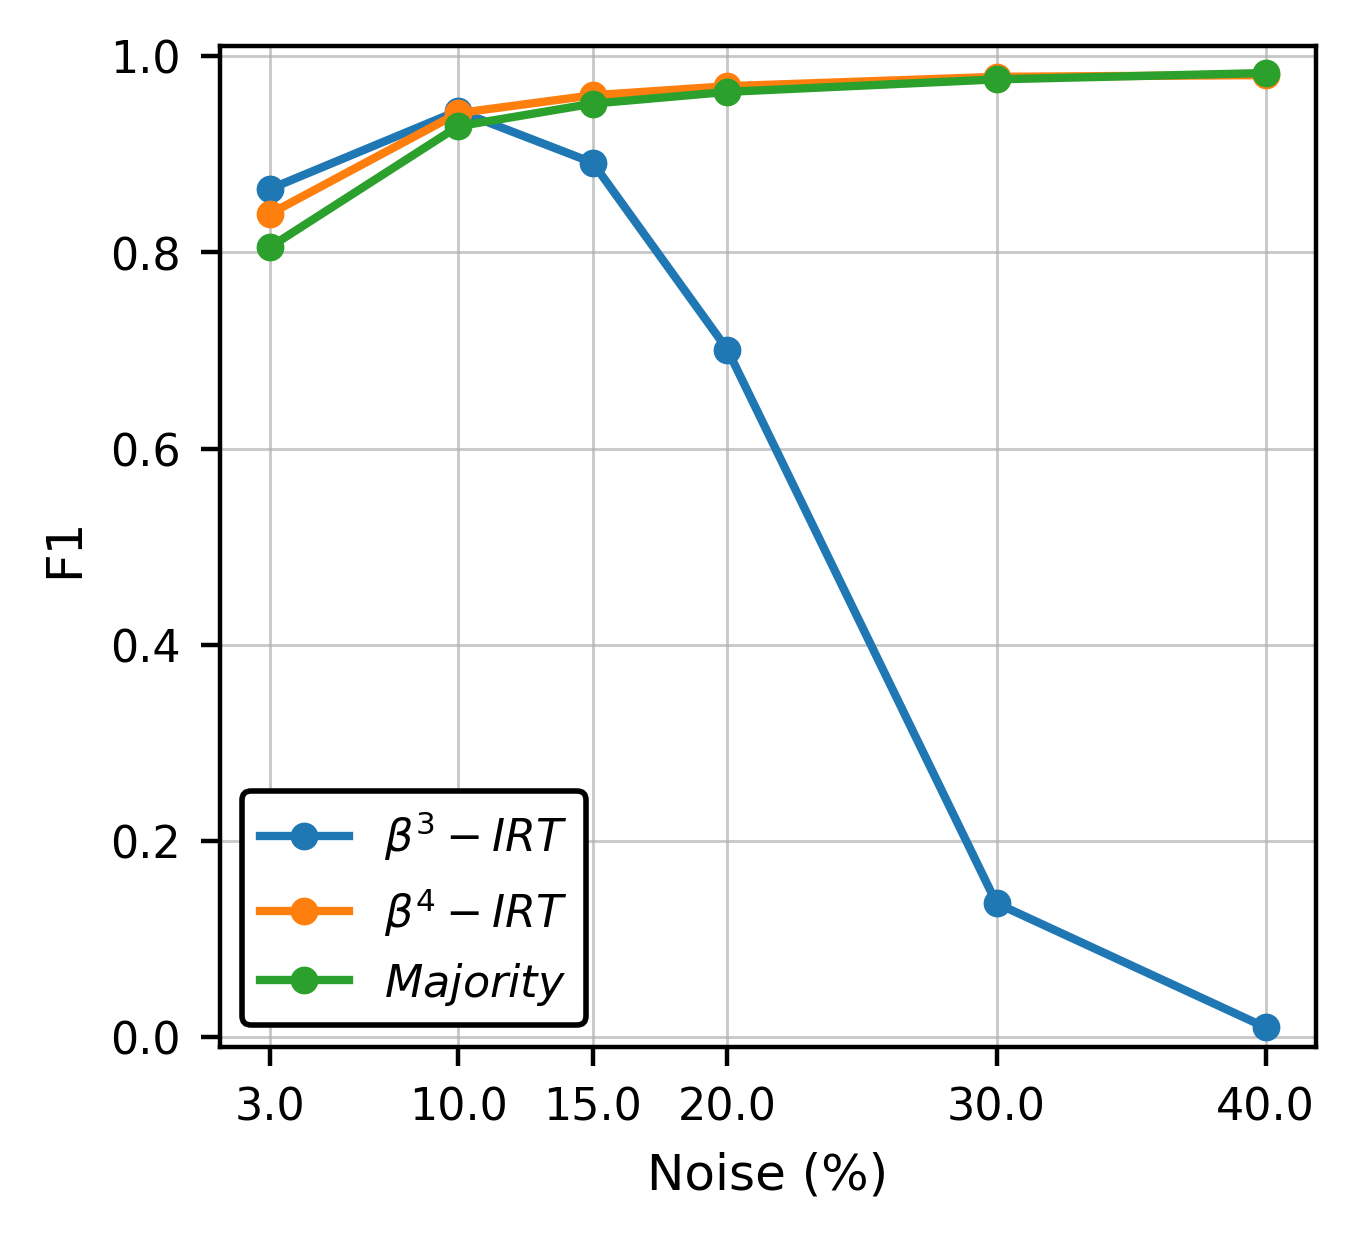
\includegraphics[width=\linewidth]{chapters/fundamentacao/imagens/02-fig_f1_noise_analysis.png}
        \caption{F1-score}
        \label{fig:grafico1}
    \end{subfigure}
    \hfill
    \begin{subfigure}{0.45\textwidth}
        \centering
        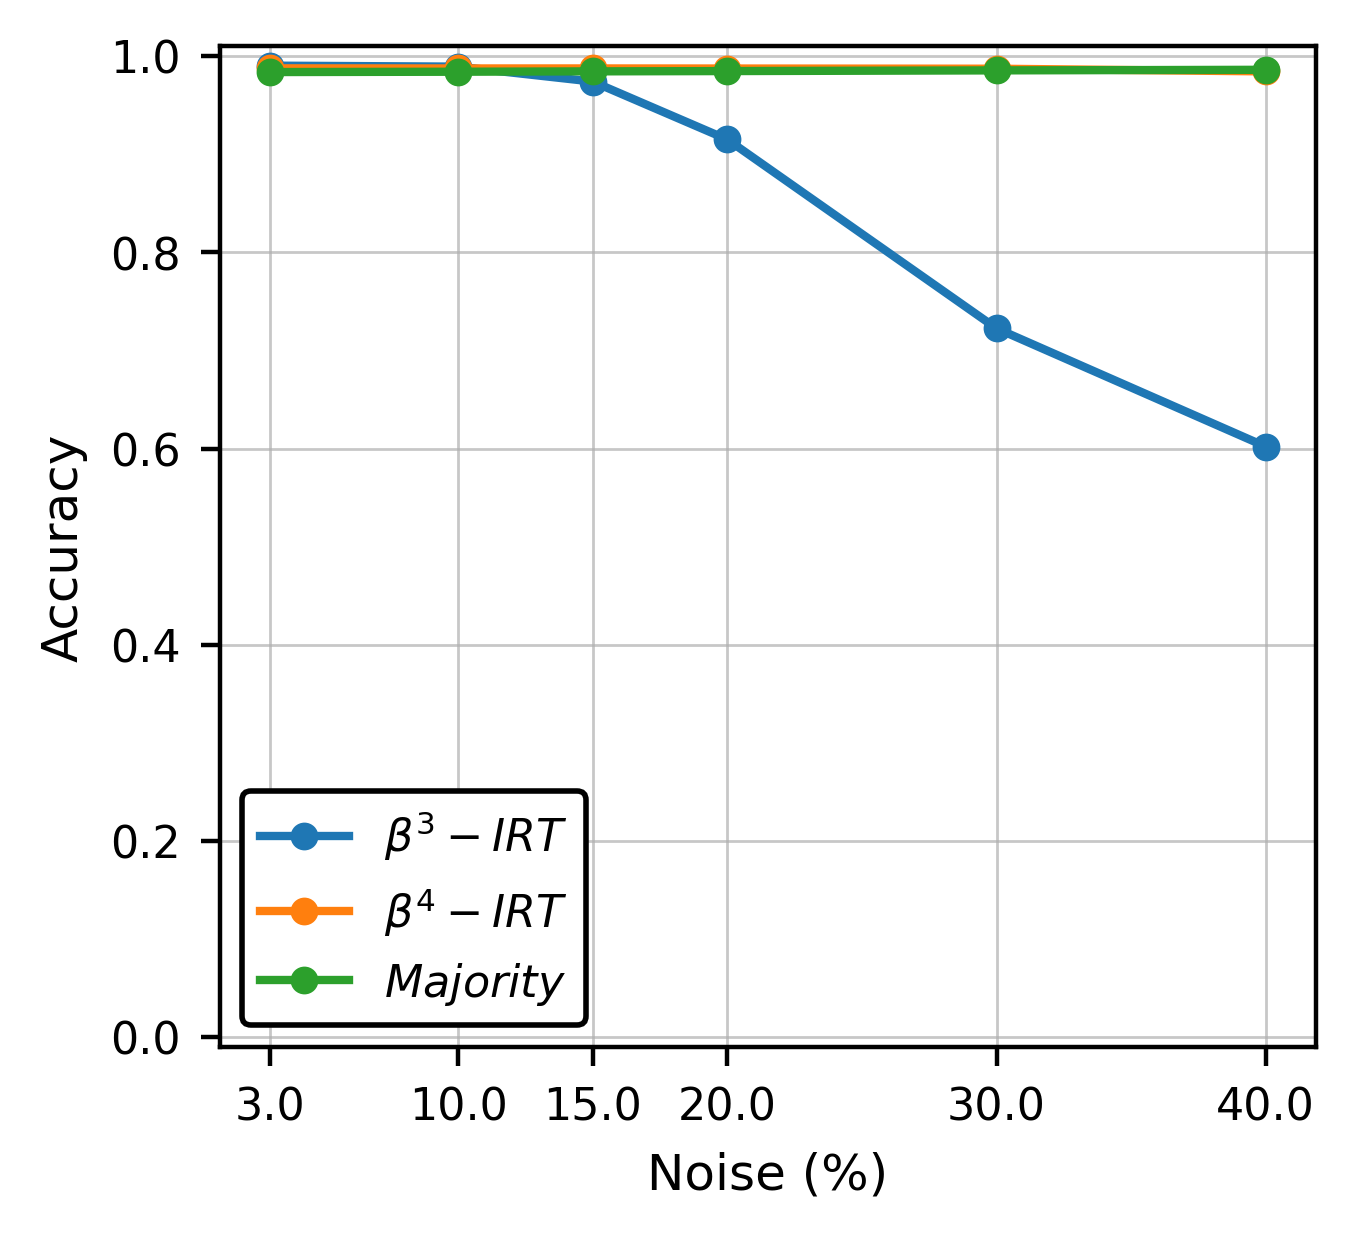
\includegraphics[width=\linewidth]{chapters/fundamentacao/imagens/02-fig_accuracy_noise_analysis.png}
        \caption{Acurácia}
        \label{fig:grafico2}
    \end{subfigure}
    
    \vspace{0.4cm}
    
    \begin{subfigure}{0.45\textwidth}
        \centering
        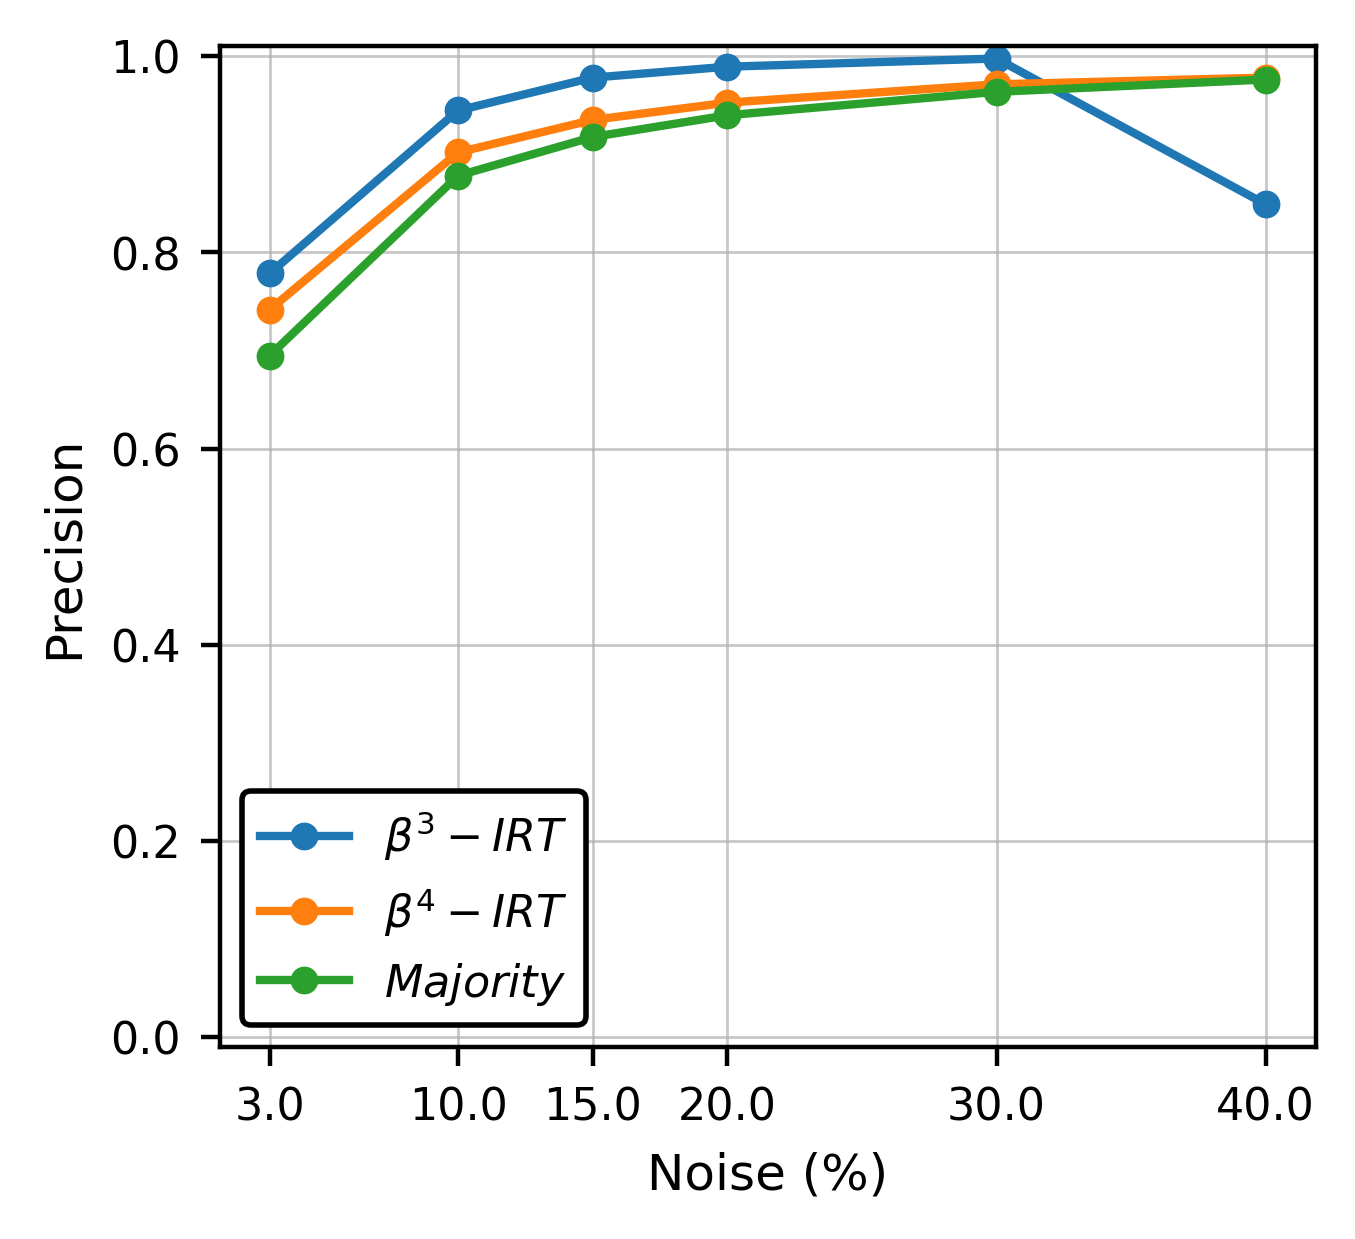
\includegraphics[width=\linewidth]{chapters/fundamentacao/imagens/02-fig_precision_noise_analysis.png}
        \caption{Precisão}
        \label{fig:grafico3}
    \end{subfigure}
    \hfill
    \begin{subfigure}{0.45\textwidth}
        \centering
        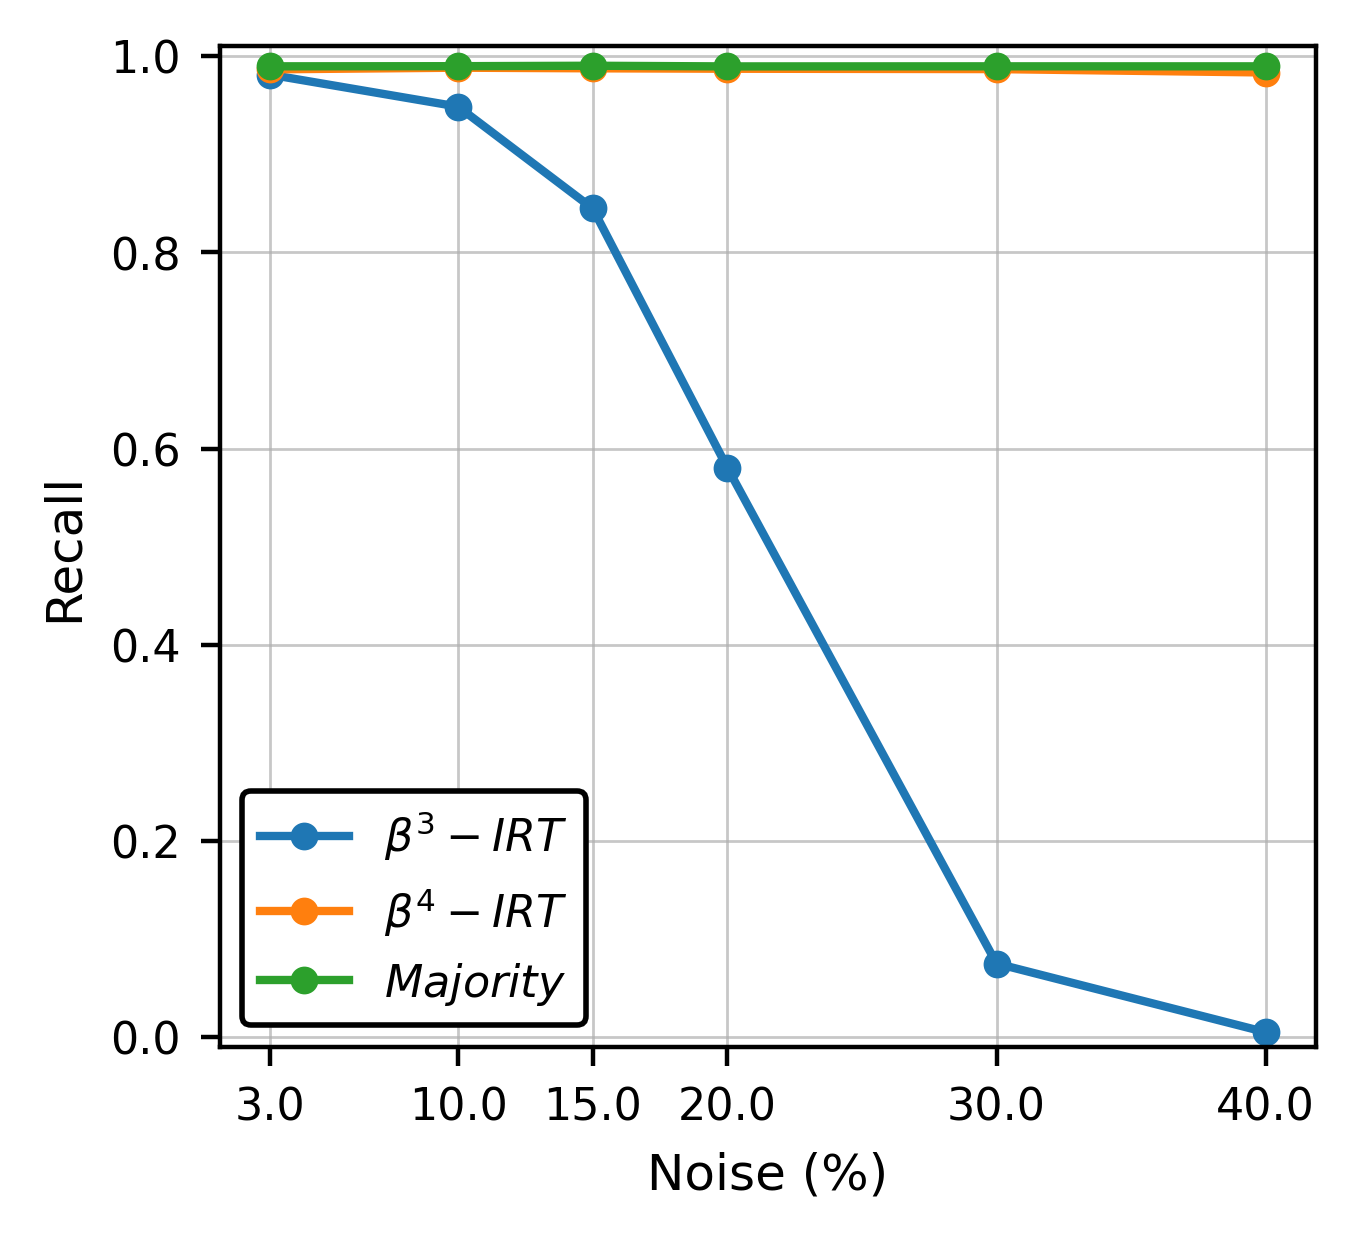
\includegraphics[width=\linewidth]{chapters/fundamentacao/imagens/02-fig_recall_noise_analysis.png}
        \caption{Recall}
        \label{fig:grafico4}
    \end{subfigure}
    
    \caption{Métricas de desempenho para cada percentual de introdução de ruído.}
    \label{fig:performances-vs-majority}
\end{figure}

A Figura \ref{fig:performances-vs-majority} apresenta os resultados em termos de F1-score, acurácia, precisão e recall para diferentes níveis de ruído. Em cenários com baixa proporção de rótulos corrompidos (entre 3\% e 10\%), ambos os modelos IRT apresentam desempenhos muito semelhantes, superando consistentemente o Majority Voting em todas as métricas avaliadas. Nesse regime, observa-se que o $\beta^{3}$-\gls{IRT} tende a identificar um número menor de instâncias como ruidosas (menor recall), mas com ligeiro ganho em precisão, indicando um comportamento mais conservador na detecção.

À medida que a proporção de ruído aumenta, o desempenho do $\beta^{3}$-\gls{IRT} se deteriora progressivamente, enquanto o $\beta^{4}$-\gls{IRT} mantém maior estabilidade e passa a superar o $\beta^{3}$-\gls{IRT} de forma mais evidente. Esse comportamento sugere que o $\beta^{4}$-\gls{IRT} apresenta maior robustez em cenários com níveis mais elevados de corrupção, conseguindo preservar melhor a capacidade de identificar instâncias inconsistentes.


\begin{figure*}[!htb]
\centering
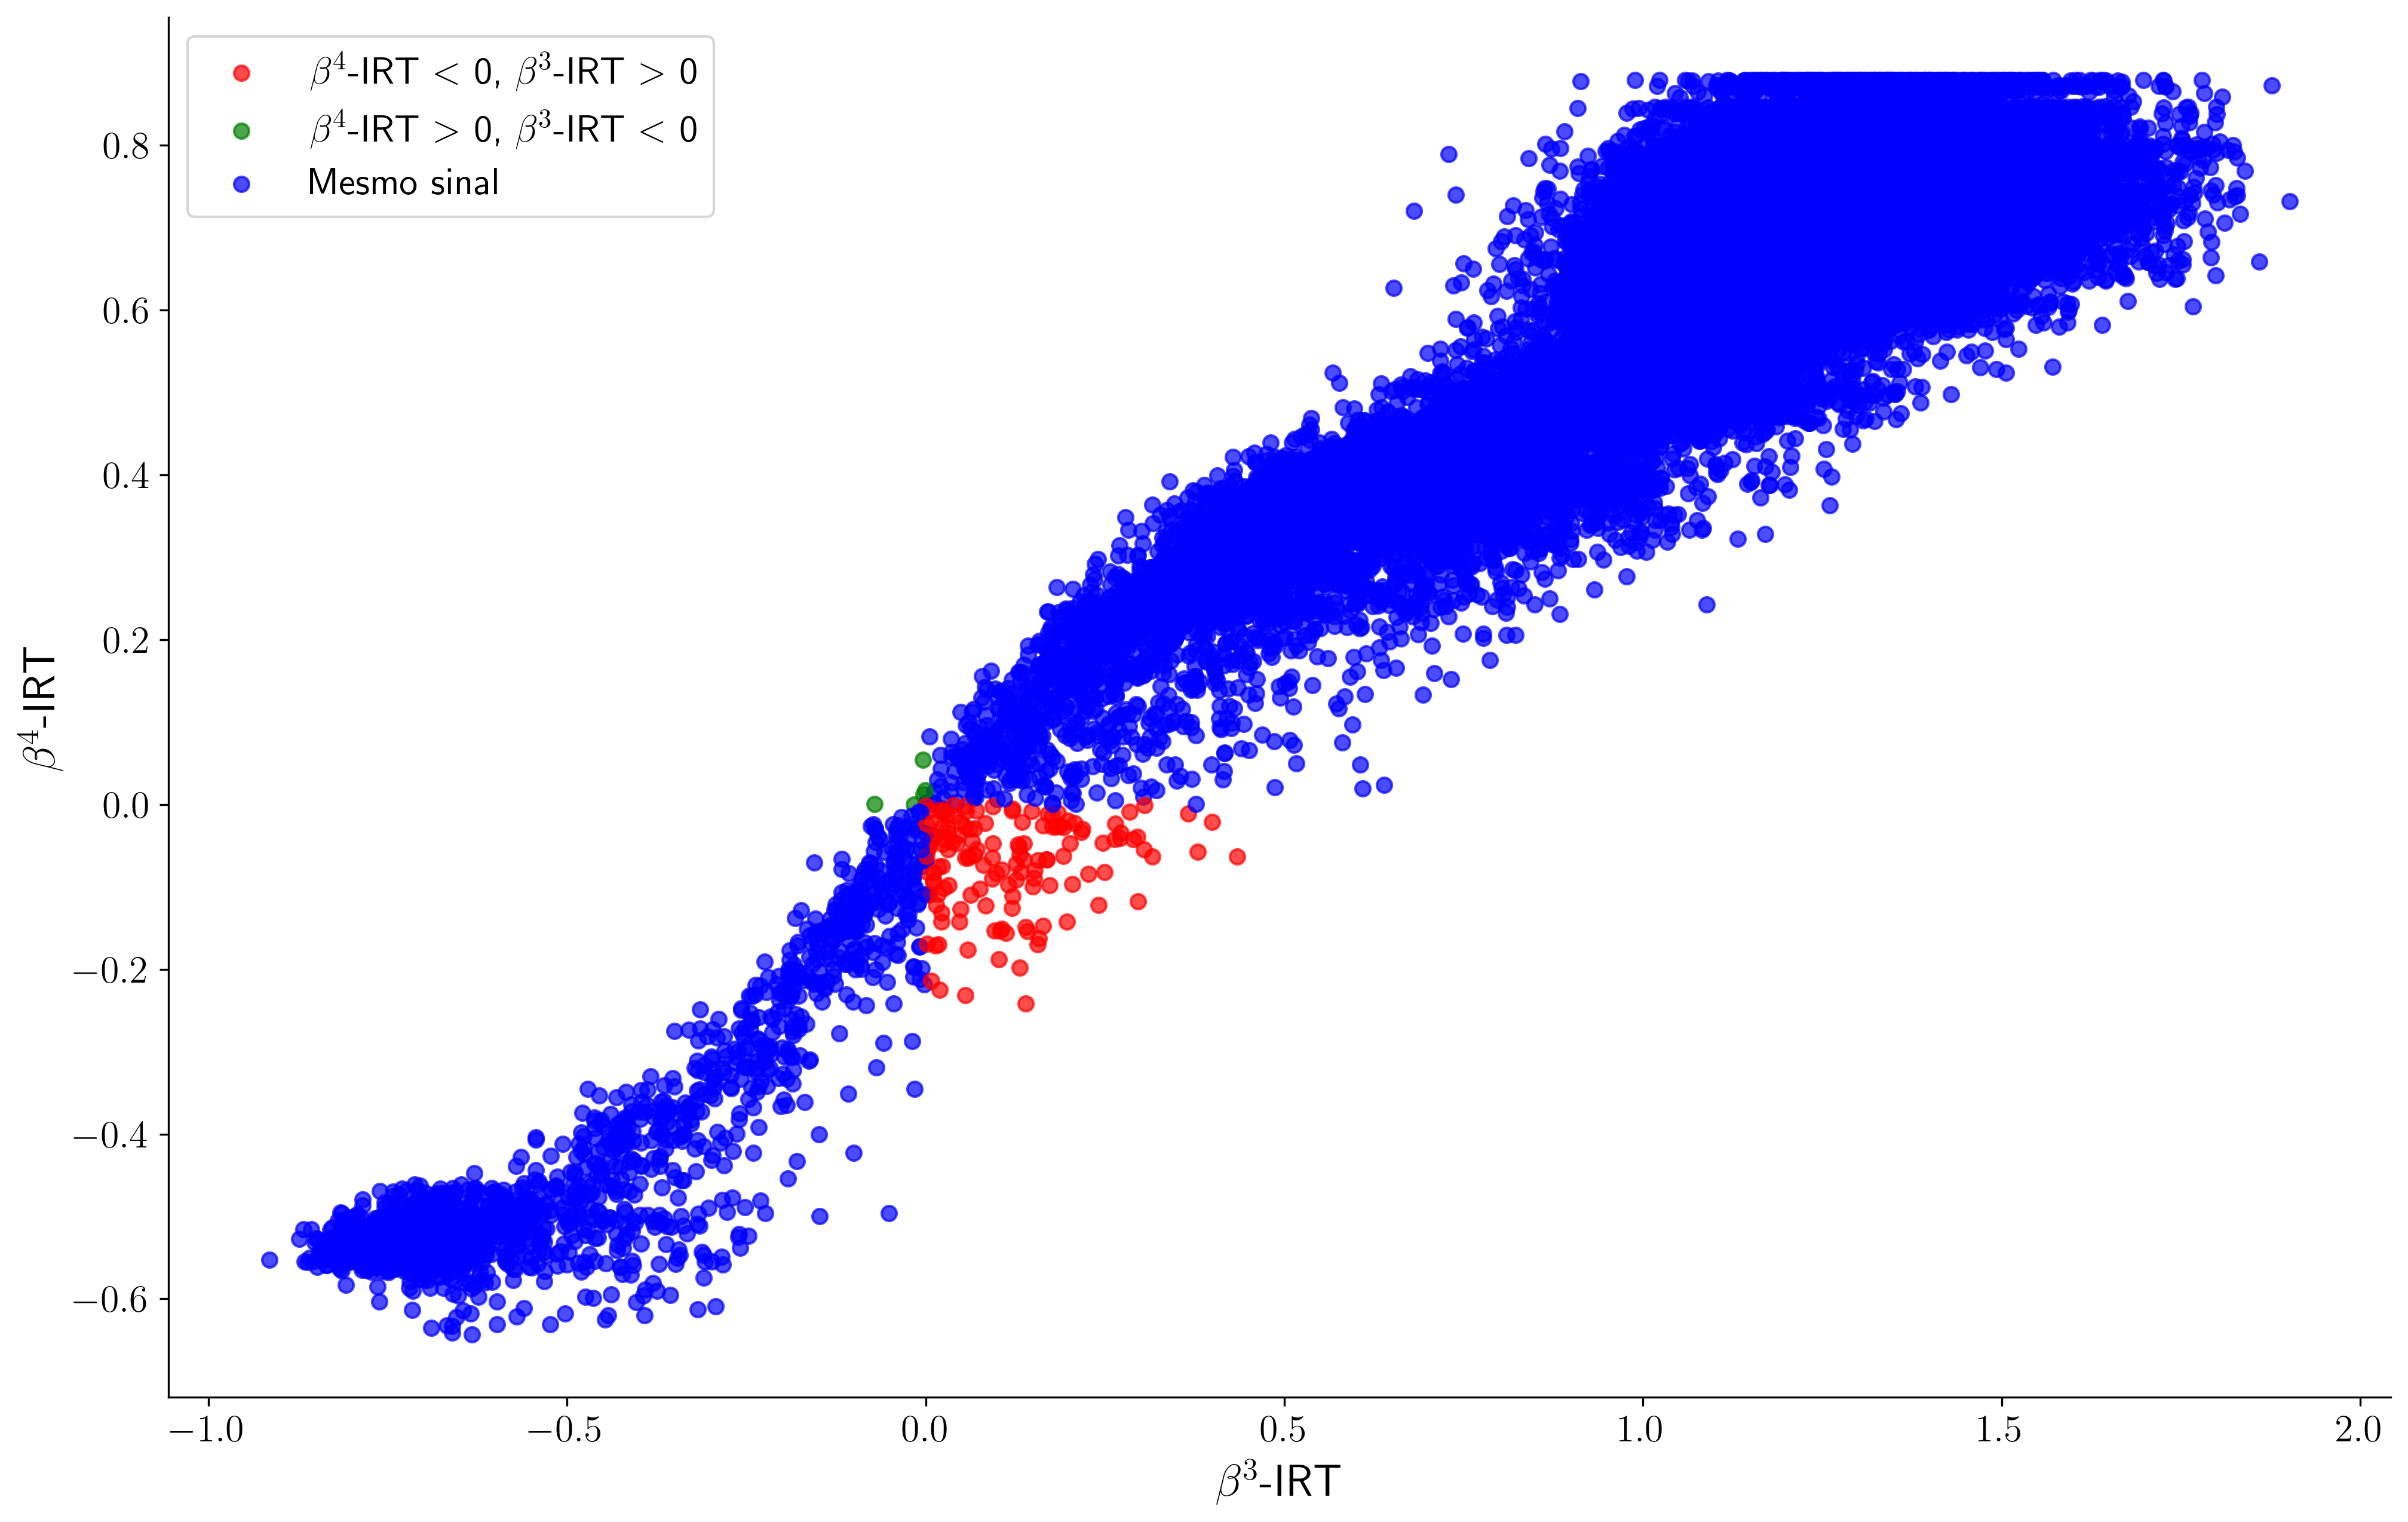
\includegraphics[width=\linewidth,clip]{chapters/fundamentacao/imagens/scatter_disc_b3-e5000_i0xb4-e5000_i0_0.0_0.03.png}
%\\
%
\caption{Todas as discriminações estimadas pelo $\beta^{4}$-\gls{IRT} e pelo $\beta^{3}$-\gls{IRT}, considerando 3\% de ruído adicional nos rótulos. As divergências quanto ao sinal estimado tendem a ocorrer quando as magnitudes das discriminações são pequenas. }
\label{fig:b4-discs-0.0_0_03.png}
\end{figure*}

A Figura \ref{fig:b4-discs-0.0_0_03.png} ilustra a comparação entre as discriminações estimadas pelos dois modelos em um cenário com 3\% de ruído. Observa-se que as diferenças de sinais concentram-se majoritariamente em instâncias com magnitude de discriminação próxima de zero. Essas instâncias correspondem a itens com baixa contribuição para a estimação das habilidades latentes, o que explica a sensibilidade do $\beta^{3}$-\gls{IRT} nesses casos. Por outro lado, o $\beta^{4}$-\gls{IRT} demonstra maior estabilidade na preservação do sinal, reforçando a evidência empírica observada nas métricas globais. De forma geral, os resultados indicam que o $\beta^{4}$-\gls{IRT} não apenas iguala ou supera o \textit{Majority Voting} em todos os níveis de ruído, como também apresenta maior robustez em comparação ao $\beta^{3}$-\gls{IRT}, especialmente em cenários com alta proporção de rótulos ruidosos.


\section{Conclusão}

Os experimentos apresentados neste capítulo evidenciam que o problema de simétria do $\beta^{3}$-\gls{IRT} impacta diretamente a recuperação consistente dos parâmetros latentes. A análise gráfica demonstrou que a inversão de sinais nas discriminações gera efeitos compensatórios nas dificuldades e, consequentemente, nas habilidades estimadas, produzindo dispersões significativas em relação aos valores verdadeiros. Ainda que estratégias de inicialização reduzam parcialmente esse fenômeno, elas não eliminam sua causa estrutural, uma vez que a não-identificabilidade permanece inerente à parametrização original do modelo.

A reformulação introduzida no $\beta^{4}$-\gls{IRT}, ao separar explicitamente magnitude e sinal do parâmetro de discriminação, permite impor restrições mais informativas e estruturalmente coerentes durante o processo de estimação. Os experimentos ilustrativos mostraram que, embora a simples decomposição não elimine automaticamente a simétria, a incorporação de priors sensíveis reduz drasticamente a ocorrência de inversões de sinal e melhora a estabilidade global do modelo.

% Os resultados do experimento de Monte Carlo reforçam essas conclusões.
Em múltiplas configurações de dados, o $\beta^{4}$-\gls{IRT} apresentou recuperação consistentemente superior do parâmetro de dificuldade e praticamente eliminou o problema de inversão de sinais nas discriminações. A  maior incidência de sinais invertidos por base do $\beta^{3}$-\gls{IRT} compromete a consistência interpretativa dos parâmetros associados aos itens. A redução expressiva nas inversões observada no $\beta^{4}$-\gls{IRT} teve impacto direto na melhoria da estimação das dificuldades, evidenciando a vantagem prática da nova parametrização.

De maneira geral, os resultados indicam que o $\beta^{4}$-\gls{IRT} oferece uma estrutura mais robusta para modelagem de respostas contínuas no intervalo $(0,1)$. Ao mitigar os efeitos da simétria do modelo original, a nova formulação proporciona maior estabilidade, reduz drasticamente a ocorrência de inversões de sinal e melhora a recuperação dos parâmetros associados aos itens. O $\beta^{3}$-\gls{IRT} apresenta uma vulnerabilidade quanto ao sinal das discriminações, comprometendo a consistência global do modelo. Diante dessas evidências, optou-se por utilizar o $\beta^{4}$-\gls{IRT} como base para o desenvolvimento do método \gls{CLAIRE}, uma vez que sua parametrização mais estável e interpretável é particularmente adequada ao cenário de avaliação de modelos de agrupamento.

